\documentclass[border=10pt]{standalone}
\usepackage{tikz}
\usetikzlibrary{arrows.meta, positioning}

\tikzset{
  part/.style  = {rectangle, draw, thick, minimum width=3cm,
                  minimum height=1cm, align=center},
  leader/.style = {->, >=Stealth, thin, shorten >=2pt}
}

\begin{document}
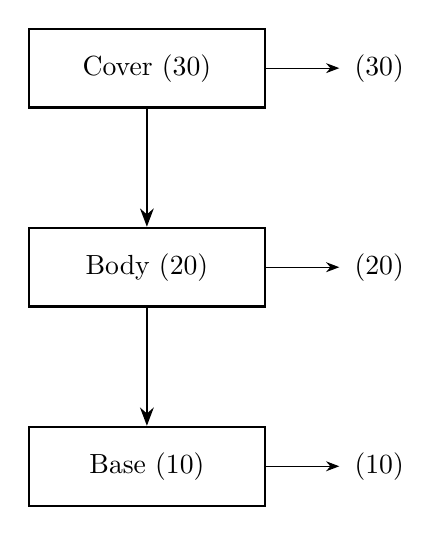
\begin{tikzpicture}[node distance=1.5cm]
  \node (top) [part]               {Cover (30)};
  \node (mid) [part, below=of top] {Body (20)};
  \node (bot) [part, below=of mid] {Base (10)};

  % 조립 방향 화살표
  \draw[->, >=Stealth, thick] (top) -- (mid);
  \draw[->, >=Stealth, thick] (mid) -- (bot);

  % 인출선 + 참조번호
  \draw[leader] (top.east) -- ++(1,0) node[right] {(30)};
  \draw[leader] (mid.east) -- ++(1,0) node[right] {(20)};
  \draw[leader] (bot.east) -- ++(1,0) node[right] {(10)};
\end{tikzpicture}
\end{document}
